\section{Multi-party computation in a nutshell}
Multi-party computation originated with the toy example presented by Yao in 1982 \cite{Yao1982ProtocolsComputations} and now known as the \emph{Millionaire's Problem}: two millionaires both want to know who is richer, but none of them want to disclose their fortune nor trust a third party. Other applications of MPC may concern electronic voting or solutions of private-data as a service (PDaaS).

+ general description of rounds etc...

\subsection{Bit-wise decomposition}
Two types: bit-wise decomposition and additive sharing. Arithmetic and boolean circuits.

\subsubsection{Oblivious transfer}
The idea behind \emph{oblivious transfer} originally described by Rabin in 1981 \cite{Rabin1981HowTransfer.} is the transfer of an information in possession of a first party and asked by a second party without the first knowing which information has been transferred. Hence, the name oblivious, or alternatively, unconscious. Different protocols exist and are all based on the \emph{RSA scheme}. 

The most common version is the \emph{1-2 oblivious transfer} \cite{Even1985AContracts} and goes as follows: Alice is in possession of two messages $m_0$ and $m_1$ and Bob wants to get message $m_p$. Alice first generates a set of private key $d$ and public key $(N,e)$ and sends two random messages $x_0$ and $x_1$ to Bob. He then generates a random message $k$ and encrypts it with the $x_i$ corresponding to the wanted message: $v = \left(x_p + k^e\right) \mod N$ and sends it to Alice. She then recovers both $k$ without knowing which one corresponds to Bob's original one: $k_i = \left(v-x_i^d\right) \mod N$. These $k_i$ then serve to encrypt the messages which are finally sent to Bob $s_i = m_i+k_i$. Bob can then only decrypt the wanted message $m_p = s_p-k$. 

This protocol has been generalised to more than two parties \cite{Ishai1997PrivateApplications,Shankar2008AlternativeTransfer,Tassa2011GeneralizedSharing}

\subsubsection{Yao's garbled circuits}
\emph{Garbled circuits} (GC) were first introduced by Yao in 1986 \cite{Yao1986HowSecrets} and now one of the most efficient solutions for generic secure two-party computation. A function has to be decomposed into a boolean circuit consisting of two-input gates (e.g. XOR and AND). Let's consider the simplest example of evaluating an AND-gate between Alice and Bob. Alice first generates a different random sequence --- also called \emph{labels} --- for each possible value of each input --- also called \emph{wires} --- and output. In the truth table, the output are then symmetrically encrypted with the hash of each corresponding input. These four resulting cyphertexts are then randomly permuted --- hence the name \emph{garbled} --- and sent to Bob. The garbling of an AND-gate is illustrated at table~\ref{tab:ang-garb}. Once Bob receives the garbled gate, he then asks Alice for her label. As they have been randomly chosen, she can send it to him without him possibly knowing what value it corresponds to. Afterwards, he also needs to know the label of his input. This part is a bit more tricky and is solved using the previously described \emph{oblivious transfer}. Bob can now compute the hash of the two labels and decrypt each element of the garbled gate until we find one corresponding with the garbled gate he recieved from Alice. He can then reveal the value to Alice either she can reveal the mapping of the garbling. The same principle can be used on a multi-gate circuit by garbling the sole end result.

\begin{figure}
        \begin{subfigure}[b]{.32\textwidth} 
            \centering 
            \begin{tabular}{IC{.6cm}|C{.6cm}IC{1.3cm}I}
            \hlineI
            A & B & output \\ \hlineI
            0 & 0 & 0  \\ \hline
            1 & 0 & 0 \\ \hline
            0 & 1 & 0 \\ \hline
            1 & 1 & 1 \\ \hlineI
            \end{tabular}
            \caption{Truth table.} 
        \end{subfigure}
        \hfill
        \begin{subfigure}[b]{.32\textwidth} 
            \centering 
            \begin{tabular}{IC{.6cm}|C{.6cm}IC{1.3cm}I}
            \hlineI
            A & B & output \\ \hlineI
            $x_A^0$ & $x_B^0$ & $x_{\textnormal{output}}^0$ \\ \hline
            $x_A^1$ & $x_B^0$ & $x_{\textnormal{output}}^0$ \\ \hline
            $x_A^0$ & $x_B^1$ & $x_{\textnormal{output}}^0$ \\ \hline
            $x_A^1$ & $x_B^1$ & $x_{\textnormal{output}}^1$ \\ \hlineI
            \end{tabular}
            \caption{Labelled truth table.} 
        \end{subfigure}
        \hfill
        \begin{subfigure}[b]{.32\textwidth}
            \centering 
            \begin{tabular}{IC{3.2cm}I}
            \hlineI
            output \\ \hlineI
            $\mathscr{E}_{H\left(x_A^1,x_B^0\right)}\left(x_{\textnormal{output}}^0\right)$ \\ \hline
            $\mathscr{E}_{H\left(x_A^1,x_B^1\right)}\left(x_{\textnormal{output}}^1\right)$ \\ \hline
            $\mathscr{E}_{H\left(x_A^0,x_B^0\right)}\left(x_{\textnormal{output}}^0\right)$ \\ \hline
            $\mathscr{E}_{H\left(x_A^0,x_B^1\right)}\left(x_{\textnormal{output}}^0\right)$ \\ \hlineI
            \end{tabular}
            \caption{Garbled output.} 
        \end{subfigure}
        \captionof{table}{Garbling of the AND-gate.}
        \label{tab:ang-garb}
\end{figure}

It is interesting to note that the secure evaluation of a sole AND-gate does not respect the principles of the multi-party computation, by definition of the AND-gate. Indeed, if the final solution is 1, both players know their respective input value, which is thus disclosed\footnote{This is not the case for the XOR-gate as an 1-output has two corresponding inputs possible, as has the 0-output}. Therefore, the total functions evaluated have to be totally surjective for each input. The circuit corresponding to the Millionaire's problem is given at figure~\ref{c2:yao-comp} and while it consists of AND-gates, the function is totally subjective with respect to each millionaire's fortune.

\begin{figure}[ht!]
    \centering
    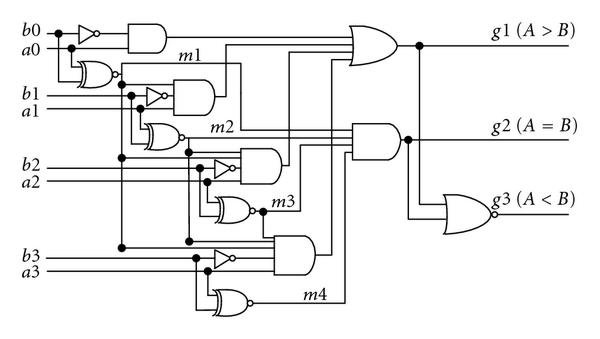
\includegraphics[width=.7\textwidth]{parts/chap-3/img/yao-comp.jpg}
    \caption{The figital comporator is the boolean circuit used to soleve Yao's millionnaire problem.} 
    \label{c2:yao-comp}
\end{figure}

This protocol executes in polynomial time, but there exists a lots of optimisations that allow to garble and evaluate the gates more rapidly.

\subsubsection{GMW protocol}
The \emph{Goldreich-Micali-Widgerson} (GMW) protocol can be seen as an extension of garbled circuits to multiple parties using Yao's idea of using oblivious transfer \cite{Goldreich1987HowGame}. The main principles here are based upon bit-sharing: each party shares its input bits among the $n$ players $b = \sum_{i=1\ldots n}b_i \mod 2$. Each player then processes their shares among the circuit. XOR-gates are easy as they can just addition the shares $c_i = a_i + b_i$. However AND-gates are more tricky: we can see from the decomposition that $c = a \cdot b = \sum_{i\neq j}a_ib_j+\sum_{1\leq i< j\neq n}\left(a_ib_j + a_jb_i \right) \mod 2$. By consequence, each party will have to compute $a_ib_i+ \sum_{i\neq j}\left( a_ib_j + a_jb_i\right)$. As for the XOR-gate, the first part is trivial to evaluate, however, the second cannot be computed by party $i$ without more information from party $j$. This is solved by using a variant of garbled circuits with oblivious transfer between parties $i$ and $j$.

\subsection{Avoiding bit-wise decomposition}
Alternatively, some arithmetic circuits can also be used for multi-party computation. The problem of the bit-wise decomposition and the use of the boolean circuit transcription of the function we jointly want to evaluate is their expensiveness in terms of performance. Indeed, a simple operation can rapidly lead to a lot of gates. For example, let's consider the addition of two number: for two numbers of $n$ bits, the total number of gates is $5n$ in a full adder composition. This is even worse for multiplication. Of course, some optimisations can be made, but the general number of gates is very high compared to the arithmetic circuit of the same function, where it would just be one single gate for addition and multiplication. We will see later that MPC over arithmetic circuits has a much higher \emph{round complexity} --- the dependence of the different rounds on each other --- which leads to less possible parallelisation than with boolean circuits. Nevertheless, one can argue that the parallelisation of bit-wise decomposition does not compensate the much higher number of gates and is thus less efficient than arithmetic circuits in general \cite{Aly2018PracticallyBit-Decomposition}.

+ general comparison of bit-wise decomposition performance and additive secret sharing comparison \cite{Blom2014AThesis}.

Comparisons are much more feasible in boolean circuits.

\subsubsection{How to share a secret}
The building block of multi-party computation over arithmetic is based upon secret sharing. Each party computes its own version of the circuit with the shares of the different parties. At the end of the circuit processing, each party has a share of the final output, which can then be put together to obtain the final output. We first have to define a way for a party to share its secret among $n$ parties, including itself.

\paragraph{Additive secret sharing}
The simplest idea is just to divide the secret $a$ in $n$ shares $a_i$ using a simple summation: $a = \sum_{i=1 \ldots n}a_i$. However, doing it in this manner allows the shares to release some information about the secret, as the shares are not random and strongly depend on the secret. They are two solutions to this problem and the first one is to consider additive sharing over $\mathbb{Z}_q$. The sharing now becomes $a = \sum_{i=1\ldots n}a_i \mod q$ which solves the problem, as the shares can now really be chosen at random. The other solution is over $\mathbb{Z}$ and consists in choosing a sufficiently large interval in which the shares are chosen to dilute sufficiently the statistical information about the secret, typically $a_i \in \left[-A2^\rho,A2^\rho\right]$ with $A$ the size of the interval of the secret $a \in \left[-A,A\right]$ and typically $\rho=128$.

Another consequence of this scheme is that all parties are vital to the recovery of secret as a loss of one secret unables us to reconstruct the secret or any statistical information about it as we took care of that. The scheme does not tolerate the loss or treason of one party and is therefore very sensitive to any failure or malicious player. This problem is solved by polynomial secret sharing.



\paragraph{Polynomial secret sharing}
The idea of polynomial sharing was originally proposed by Shamir in 1979 \cite{Shamir1979HowSecret}. This method allows $n$ parties to share a secret in a way such that any subset of $t+1$ parties can later reconstruct the secret but any subgroup of maximum $t$ parties can do so. The scheme is based on the single fact that for any polynomial of degree $d$, any subset of $d+1$ or more different points can reconstruct the polynomial completely whereas any subset of at most $d$ points is left with an infinite number of possibilities.

The scheme goes as follows. The party that wants to share its secret first constructs a polynomial of degree $t$.
\begin{equation}
    h(z) = a + \sum_{i=1}^t b_i z^i
\end{equation}
with secret $a$ random coefficients $b_i$. For the same reasons as for additive secret sharing, the coefficients can either be chosen in $b_i \in \mathbb{Z}_q$ (which also leads to the consideration of polynomial $h(z) \mod q$ instead), either in the interval $b_i \in \left[-A2^\rho,A2^\rho\right]$.
\noteH{should I demonstrate ?}

We verify that $h(0)=a$ and distribute shares $a_i$ to each party $i$ --- including ourselves --- as follows $a_i=h(i)$. $t+1$ parties can now reconstruct the polynomial together using e.g. Lagrange's polynomials and compute $f(0)$ to recover the secret share. An interesting property is that the recovery can be done as a simple linear combination. Indeed, we have
\begin{eqnarray*}
    h(0) &=& \sum_{i=1}^{n} l_i(0)h(i) \\
    a &=& \sum_{i=1}^{n} r_ia_i
\end{eqnarray*}
where $r = \left(r_1, \ldots , r_n\right) = \left(l_1(0), \ldots , l_n(0)\right)$ is called the \emph{recombination vector} with $l_i(z)$ the $i$-th order Lagrange polynomial, for example
\begin{equation*}
    l_i(z) = \prod_{1\leq j \leq n,j\neq i}\frac{z-j}{i-j}
\end{equation*}
This also works with any generating set of $\mathbb{Z}\left[z\right]$ (or alternatively $\mathbb{Z}_q\left[z\right]$), as long all parties use the same set.

\subsubsection{Performing basic operations}

\paragraph{Addition and multiplication of public constants}
Each party just adds or multiplies his share with the constant. This rests on some arithmetic properties of polynomials: one can easily verify that $a_i+c$ is a share of $a+c$ and $c \cdot a_i$ of $c \cdot a$.

\paragraph{Addition of two secrets}
Let's consider the addition of two polynomials: the respective coefficients just add up. By consequence, two secrets $a$ and $b$ can be added up if every party adds their local shares $a_i+b_i$.
\noteH{False, the values $h(i)$ are added up, not the coefficients}


\paragraph{Multiplication of two secrets}
Unfortunately, it is not possible to adopt the same strategy for multiplication as the multiplication of two polynomials of order $t$ will lead to a new polynomial of order $2t$ which will double the number of parties needed to recover the secret output. In real-case functions with a lot of multiplications, this becomes rapidly impracticable and theoretically unsolvable if the degree of the new polynomial exceeds $n$. Another problem is of statistical order: the new polynomial is not random anymore as it is for example not irreducible anymore by construction. Different algorithms exist to solve this problem \noteH{cite different algorithms ?}

\paragraph{Exponentiation}


\paragraph{Boolean operations}